\documentclass[lettersize,journal]{IEEEtran}
\usepackage{amsmath,amsfonts}
\usepackage{algorithmic}
\usepackage{algorithm}
\usepackage{array}
\usepackage[caption=false,font=normalsize,labelfont=sf,textfont=sf]{subfig}
\usepackage{textcomp}
\usepackage{stfloats}
\usepackage{url}
\usepackage{verbatim}
\usepackage{graphicx}
\usepackage{cite}
\usepackage{tikz}
\usepackage{pgf-pie}
\hyphenation{op-tical net-works semi-conduc-tor IEEE-Xplore}
% updated with editorial comments 8/9/2021

\begin{document}

\title{Pengetahuan dan Kemampuan yang Dimiliki Pengguna Non-Ahli dalam Mendeteksi Phishing}

\author{IEEE Publication Technology,~\IEEEmembership{Adhi Wahyu Utama and Dimas Anwar Aziz,~Telkom University,}
  % <-this % stops a space
  \thanks{This paper was produced by the IEEE Publication Technology Group. They are in Piscataway, NJ.}% <-this % stops a space
  \thanks{Manuscript received April 19, 2021; revised August 16, 2021.}
}

% The paper headers
\markboth{Journal of \LaTeX\ Class Files,~Vol.~14, No.~8, August~2021}%
{Shell \MakeLowercase{\textit{et al.}}: A Sample Article Using IEEEtran.cls for IEEE Journals}

% \IEEEpubid{0000--0000/00\$00.00~\copyright~2021 IEEE}
% Remember, if you use this you must call \IEEEpubidadjcol in the second
% column for its text to clear the IEEEpubid mark.

\maketitle

\begin{abstract}
  Email phishing adalah komunikasi penipuan yang berpura-pura menjadi sesuatu
  yang bukan sebenarnya untuk membuat orang melakukan tindakan yang seharusnya
  tidak mereka lakukan. Kami melakukan survei terhadap beberapa orang dari
  berbagai demografi di Indonesia dan meminta mereka untuk berbagi pengalaman
  mereka terkait email phishing. Dari analisis pengalaman tersebut, kami menemukan
  bahwa cara pengguna email mendeteksi pesan phishing memiliki banyak kesamaan
  dengan cara ahli IT mengidentifikasi phishing. Kami juga menemukan bahwa pengguna
  email memiliki pengetahuan unik dan kemampuan berharga dalam proses identifikasi
  yang tidak dimiliki oleh kontrol teknis maupun ahli IT. Kami menyarankan bahwa
  pelatihan yang ditargetkan pada cara memanfaatkan keunikan ini kemungkinan akan
  meningkatkan pencegahan phishing.
\end{abstract}

\begin{IEEEkeywords}
  Phishing detection, non-expert users, email security, user capabilities, cybersecurity awareness, security training, user knowledge, online threats, digital literacy, human factors in security.
\end{IEEEkeywords}

\section{Introduction}
\IEEEPARstart{E}{mail} adalah salah satu metode komunikasi yang paling umum
digunakan, terutama dalam organisasi besar dan e-commerce. Lebih dari 3,9 miliar
orang memiliki akun email, dan secara kolektif mereka mengirim dan menerima
lebih dari 290 miliar email per hari \cite{satusatu}. Email merupakan salah
satu metode utama yang digunakan untuk berkomunikasi dengan orang asing.
Namun, karena email adalah sistem global di mana siapa saja dapat berkomunikasi
dengan siapa saja, pelaku kejahatan mengirim email yang berpura-pura menjadi
sesuatu yang bukan sebenarnya, dan menipu orang untuk melakukan tindakan yang
seharusnya tidak mereka lakukan — yang dikenal sebagai phishing \cite{tigaempat}.
Pesan phishing adalah vektor serangan yang telah menyebabkan banyak kerugian
dalam masyarakat. Email phishing telah digunakan untuk mencuri uang dalam jumlah
besar \cite{duadua}, menginstal ransomware \cite{tigasatu}, atau sekadar mencuri
konten email yang kemudian dipublikasikan \cite{duasatu}. 32\% dari semua
pelanggaran perusahaan pada tahun 2018 disebabkan oleh phishing \cite{tigatiga}.
Spear-phishing – varian di mana email disesuaikan khusus dengan penerima – digunakan
oleh 65\% kelompok yang melakukan serangan siber yang ditargetkan, dan lebih umum
digunakan daripada kerentanan zero-day (hanya 23\% dari kelompok tersebut) \cite{tigadua}.

Phishing adalah masalah sosio-teknis, dan menangani masalah ini membutuhkan
kerja sama antara inovasi teknologi dan intervensi manusia. Teknologi sedang
dikembangkan untuk membantu mengidentifikasi dan menyaring pesan phishing,
tetapi teknologi ini tidak bekerja dengan akurasi 100\% dan dapat lambat
merespons inovasi baru oleh penyerang \cite{satuempat}. Administrator IT dan
pemerintah sering mencoba menghentikan phishing sebelum dimulai dengan
mengganggu situs web phishing dan pengiriman email massal \cite{satunol}.
Tetapi garis pertahanan terakhir adalah pengguna akhir; pesan phishing yang
melewati pertahanan lain masih dapat dideteksi atau diabaikan oleh pengguna
akhir untuk mencegah kerugian.

Dalam penelitian ini, kami mensurvei pengguna email tanpa pelatihan atau
keahlian IT dan menanyakan mereka tentang pengalaman spesifik dengan email
phishing yang mereka terima. Sekitar setengah dari responden survei dapat
mengidentifikasi insiden spesifik yang kemudian mereka jawab dengan pertanyaan
terperinci. Berdasarkan model Wash \cite{tigaempat} tentang bagaimana ahli IT
mendeteksi email phishing, kami menanyakan setiap orang tentang apa yang mereka
perhatikan dari email tersebut, apa yang mereka harapkan dalam email tersebut,
apa yang membuat mereka curiga terhadap email tersebut, investigasi apa yang
mereka lakukan, bagaimana mereka memutuskan apakah email tersebut sah, dan apa
yang akhirnya mereka lakukan dengan email tersebut.

Dari pertanyaan-pertanyaan ini, kami dapat mengidentifikasi pola bagaimana
pengguna email yang bukan ahli IT saat ini mengidentifikasi email penipuan
phishing di kotak masuk mereka. Sebagian besar penelitian melihat kegagalan
deteksi phishing dan apa yang perlu diperbaiki; sebaliknya kami membandingkan
non-ahli dengan para ahli Wash dan mengidentifikasi apa yang berhasil dengan
baik yang dapat kita kembangkan. Kami menemukan bahwa pengguna email sering
membawa pengetahuan unik ke proses identifikasi ini yang tidak dimiliki oleh
metode pencegahan phishing lainnya, seperti apakah email tersebut diharapkan
atau tidak dan seperti apa email seperti ini biasanya terlihat dan meminta.
Kami juga menemukan bahwa pengguna email memiliki kemampuan berharga untuk
investigasi, seperti meminta saran dari orang lain, atau memeriksa keabsahan
dengan pengirim. Secara keseluruhan, temuan ini menunjukkan bahwa pengguna
email dapat menjadi bagian penting dari ekosistem pencegahan phishing, meskipun
pelatihan phishing dapat ditingkatkan untuk fokus pada bagaimana pengguna dapat
lebih baik menggunakan pengetahuan dan kemampuan unik mereka.

\section{Previous Work}

\subsection{Mencegah Bahaya dari Phishing}
Masyarakat kita memiliki tiga bentuk pertahanan yang membantu mengidentifikasi
dan membatasi keberhasilan penipuan phishing. Pertahanan teknologi mencoba
secara otomatis mendeteksi fitur-fitur yang diketahui dari email phishing dan
memblokir atau menghapus email tersebut. Beberapa pertahanan menggabungkan
kerja komputer dan manusia dengan memperingatkan pengguna akhir tentang potensi
pesan phishing, yang kemudian diselidiki lebih lanjut oleh pengguna akhir untuk
menentukan apakah itu email phishing. Dan akhirnya, ada pertahanan manusia, di
mana penerima email diandalkan untuk mengenali email sebagai berbahaya dan
bertindak sesuai.

\subsubsection{Deteksi dan Penghapusan Otomatis}
Pendekatan deteksi dan penghapusan otomatis bertujuan untuk mengklasifikasikan
email sebagai phishing atau sah dan memblokir atau menghapusnya sebelum
pengguna akhir menemukannya. Upaya di bidang ini telah difokuskan pada
peningkatan dan menemukan cara baru untuk mengidentifikasi pesan phishing yang
masuk dan keluar menggunakan daftar hitam \cite{satunol}, heuristik [3, 13, 16,
    23], dan pembelajaran mesin [9, 29]. Pendekatan ini menyaring email berdasarkan
fitur yang diketahui yang secara konklusif mengidentifikasi email sebagai
phishing. Namun, pendekatan otomatis mengandalkan algoritma probabilistik yang
menghasilkan positif palsu, menyebabkan email sah diblokir atau dihapus. Selain
itu, pendekatan otomatis memiliki kemampuan terbatas untuk mendeteksi variasi
baru dari serangan phishing \cite{satudua} dan tidak dapat mengidentifikasi
semua email phishing yang lebih lama.

\subsubsection{Peringatan Phishing}
Peringatan phishing melengkapi teknik deteksi otomatis dengan memperingatkan
pengguna akhir tentang potensi email phishing, alih-alih memblokir atau
menghapusnya. Peringatan biasanya digunakan ketika deteksi otomatis tidak dapat
secara konklusif mengklasifikasikan email sebagai phishing \cite{dualima}.
Dalam praktiknya, peringatan telah dilaporkan meningkatkan kemampuan pengguna
akhir untuk mengidentifikasi email phishing [8, 26]. Upaya penelitian yang
sedang berlangsung di area ini telah difokuskan pada menemukan cara yang lebih
baik untuk merancang dan menyajikan peringatan kepada pengguna akhir.

Meskipun memiliki dampak positif, peringatan memiliki keterbatasan yang sama
dengan pendekatan deteksi dan penghapusan otomatis. Mereka rentan terhadap
positif palsu (menandai email sah sebagai berpotensi berbahaya) dan negatif
palsu (membiarkan email berbahaya lolos tanpa peringatan, terutama serangan
phishing zero-hour). Seperti yang dikemukakan oleh Yang et al., peringatan dan
pelatihan pengguna harus saling melengkapi untuk meningkatkan efektivitasnya
\cite{tigatujuh}.

\subsubsection{Pelatihan Pengguna}
Peneliti dan praktisi keamanan telah mengembangkan berbagai metode dan materi
untuk melatih pengguna mengidentifikasi dan bereaksi terhadap email phishing
dengan tepat. Kumaraguru et al. \cite{satusembilan} dan Caputo et al.
\cite{dua} menemukan bahwa pelatihan tertanam (yaitu materi instruksional yang
disajikan saat peserta mengklik URL dalam email phishing), yang sangat umum
digunakan di organisasi besar, meningkatkan motivasi pengguna untuk belajar dan
meningkatkan akuisisi pengetahuan. Rader et al. \cite{duatujuh} menemukan bahwa
orang juga belajar tentang penipuan phishing dan tindakan perlindungan dari
cerita tentang insiden keamanan. Wash dan Cooper \cite{tigalima} menemukan
bahwa pelatihan phishing tradisional yang berisi fakta dan saran bekerja lebih
baik ketika disajikan oleh seorang ahli, sementara cerita keamanan naratif
bekerja lebih baik ketika diceritakan oleh seorang rekan.

Pesan pelatihan phishing yang paling banyak dibagikan di seluruh pemerintah,
bisnis, dan individu mengajarkan orang untuk mengidentifikasi tanda-tanda
tertentu (misalnya alamat email pengirim, URL dalam email, tata bahasa atau
ejaan yang buruk) atau menerapkan serangkaian aturan untuk mendeteksi,
menghindari, dan melaporkan pesan phishing. Pesan pelatihan semacam itu telah
dipelajari secara ekstensif dan menunjukkan potensi untuk meningkatkan
ketahanan orang terhadap serangan phishing [4, 19]. Beberapa pesan berfokus
pada perubahan perilaku, misalnya, tidak pernah mengklik URL atau membuka
lampiran dalam email dari pengirim yang tidak dikenal.

Pesan pelatihan lainnya berfokus pada memberi tahu pengguna tentang jenis
ancaman phishing yang umum dan cara mengidentifikasinya, dengan tujuan
memanipulasi tingkat risiko dan selanjutnya tingkat ketakutan pada pengguna [5,
    20]. Beberapa peneliti berpendapat bahwa ajakan ketakutan meningkatkan niat
pengguna akhir untuk bertindak dengan aman. Namun, meskipun mampu mengubah niat
perilaku pengguna akhir \cite{lima}, ajakan ketakutan tidak memprediksi atau
menghasilkan perilaku yang aman \cite{enam}.

Pelatihan pengguna biasanya berfokus pada aspek pesan email dan mencoba
mengubah cara orang berpikir tentang pesan email sehingga mereka memperhatikan
fitur yang paling terkait dengan phishing. Studi telah menunjukkan bahwa ini
meningkatkan pengetahuan pengguna, meningkatkan kemampuan mereka untuk
mengidentifikasi email phishing, dan mengurangi jumlah serangan yang berhasil
  [2, 19, 35]. Namun, jumlah serangan phishing yang berhasil masih cukup tinggi,
mencapai 32\% dari semua pelanggaran perusahaan pada tahun 2018. Lebih banyak
yang perlu dilakukan untuk meningkatkan kemampuan pengguna akhir dalam
mengidentifikasi dan mencegah serangan phishing.

Sebagian besar pelatihan pengguna dikembangkan dari pemahaman tentang bagaimana
dan mengapa orang jatuh ke dalam phishing \cite{enam}. Kami berhipotesis bahwa
jika pelatihan lebih fokus pada aspek bagaimana orang sudah berpikir tentang
dan menangani email secara umum, ini dapat membuka jalan baru untuk pelatihan
phishing. Sayangnya, kami tidak memiliki pemahaman yang komprehensif tentang
bagaimana pengguna non-ahli melakukannya. Masalah serupa dihadapi dalam
pelatihan keterampilan teknis di mana peneliti menyelidiki cara untuk
meningkatkan pelatihan pemecah masalah (teknisi) \cite{satulima}. Mereka
mempelajari dan mengidentifikasi proses konseptual umum dan strategi yang
digunakan teknisi saat memecahkan masalah. Ini membantu mereka mengidentifikasi
kesenjangan dalam metode dan pesan pelatihan yang ada dan selanjutnya membantu
mereka mengidentifikasi area perbaikan. Kami berpendapat bahwa memahami proses
dan strategi yang digunakan non-ahli untuk mengidentifikasi email phishing
dapat mengungkapkan area potensial untuk perbaikan pelatihan phishing.

\subsection{Bagaimana Orang Mengidentifikasi Email Phishing?}

Downs et al. \cite{tujuh} menyelidiki strategi keputusan pengguna komputer
non-ahli ketika menghadapi email yang mencurigakan. Mereka mengidentifikasi
tiga strategi yang digunakan peserta untuk memahami email yang mereka terima:
1) email ini tampaknya ditujukan untuk saya; 2) normal untuk mendengar dari
perusahaan yang Anda lakukan bisnis dengannya dan 3) perusahaan terkemuka akan
mengirim email. Downs et al. \cite{tujuh} menyatakan bahwa tidak ada strategi
yang membantu orang mengidentifikasi pesan phishing yang dirancang dengan baik.
Namun, studi tersebut melibatkan peran bermain dalam lingkungan yang
terkendali. Kami tidak tahu strategi mana yang berlaku dan seberapa umum mereka
dalam konteks alami dan kotak masuk orang.

Wash \cite{tigaempat} melihat bagaimana ahli mengidentifikasi email phishing
dengan mewawancarai 21 ahli IT tentang kejadian ketika mereka berhasil
mengidentifikasi email sebagai phishing di kotak masuk mereka. Dia
mengidentifikasi proses 3 tahap untuk mengidentifikasi email phishing. Pada
tahap pertama, email diterima dan diperlakukan seperti email lainnya — konten
dalam email diambil secara harfiah dan orang tersebut mencoba memahami email
dan mencari tahu apa yang diminta untuk dilakukan. Saat mereka melakukan ini,
mereka memperhatikan ketidaksesuaian — hal-hal yang "terasa aneh" tentang email
tersebut. Akhirnya, sesuatu memicu orang tersebut untuk berpikir bahwa email
ini tidak sah — bahwa itu mungkin email phishing yang bukan seperti yang
dikatakannya. Pada titik ini, mereka menjadi curiga dan mulai secara eksplisit
mencari hal-hal yang dapat membantu mereka menentukan apakah email tersebut sah
atau tidak. Potongan informasi baru ini sering memungkinkan mereka untuk secara
konklusif mengidentifikasi email sebagai phishing.

Pekerjaan Wash \cite{tigaempat} menunjukkan bagaimana beberapa pelajaran dari
pelatihan phishing diterapkan dalam konteks dunia nyata. Namun, Wash hanya
mempelajari para ahli. Para ahli mungkin memiliki keterampilan, pengalaman, dan
pengetahuan yang lebih maju tentang phishing dan tindakan pencegahan
dibandingkan dengan non-ahli. Kami tidak tahu temuan mana yang mungkin berlaku
untuk non-ahli dan dapat digunakan untuk meningkatkan pelatihan mereka.

\subsection{Phishing: Masalah Sosio-Teknis}

Phishing adalah masalah sosio-teknis. Solusi otomatis tidak mendeteksi 100\%
email phishing. Oleh karena itu, pengguna akhir harus mengidentifikasi email
ini di kotak masuk mereka. Seperti yang dikatakan oleh Khonji et al., tidak ada
solusi tunggal yang ada untuk mengurangi serangan phishing \cite{satutujuh};
sehingga teknik otomatis / peringatan dan pelatihan pengguna harus diterapkan
untuk saling melengkapi \cite{satusembilan}. Ini sebanding dengan Model Keju
Swiss (SCM) James Reason \cite{duadelapan} tentang penyebab dan respons
kecelakaan. SCM adalah alat populer yang digunakan untuk menyelidiki atau
menganalisis kompleksitas sistem dengan menunjukkan bahwa suatu insiden adalah
hasil dari kombinasi kegagalan aktif oleh operator dan kondisi laten dari
sistem. SCM menggambarkan sistem sosio-teknis sebagai beberapa irisan keju
Swiss yang ditumpuk bersama, masing-masing irisan dengan lubang. Setiap irisan
menggambarkan lapisan pertahanan sistem terhadap jenis kegagalan tertentu,
sementara setiap lubang mewakili kegagalan dalam pertahanan sistem pada lapisan
tertentu. Bryans dan Arief menerapkan model tersebut untuk memahami lapisan
keamanan dan toleransi kesalahan dalam sistem komputer \cite{satu}. Mereka
menggambarkan setiap lapisan sebagai mekanisme perlindungan terhadap jenis
serangan tertentu, tetapi memiliki kelemahan (lubang) terhadap jenis lainnya.

Baik teknik deteksi dan penghapusan otomatis maupun peringatan mengandalkan
pengguna akhir sebagai garis pertahanan terakhir terhadap phishing. Namun,
jumlah serangan phishing yang berhasil baru-baru ini menunjukkan bahwa lebih
banyak pekerjaan perlu dilakukan untuk meningkatkan pelatihan pengguna.
Sementara sebagian besar pelatihan berfokus pada mengajarkan pengguna akhir
untuk mengidentifikasi fitur yang diketahui dan konklusif dari email phishing,
Downs et al. \cite{tujuh} dan Wash \cite{tigaempat} menemukan bahwa pengguna
akhir mengandalkan fitur selain pembeda konklusif untuk mengidentifikasi email
phishing. Kita perlu mengeksplorasi cara-cara yang lebih baik untuk menjaga
pengguna dalam lingkaran pertahanan terhadap serangan phishing. Lebih banyak
penelitian perlu dilakukan untuk memahami bagaimana non-ahli mengidentifikasi
email phishing, aspek atau informasi apa yang mereka andalkan, dan jenis hal
yang mereka lakukan dalam proses tersebut. Pemahaman ini dapat membantu kita
menyesuaikan dan menargetkan pelatihan phishing dan teknologi yang mendukung
pengambilan keputusan manusia. Studi kami mengambil langkah pertama ke arah ini
dengan menerapkan model Wash dalam survei untuk mempelajari teknik yang diikuti
non-ahli untuk mengidentifikasi email phishing.

\section{Methods and Sample}

Dalam makalah ini, kami melihat bagaimana pengguna non-ahli mengidentifikasi
email phishing, dan melihat apakah beberapa teknik yang diidentifikasi oleh
Wash \cite{tigaempat} pada ahli juga ada ketika non-ahli mengidentifikasi email
phishing. Untuk mempelajari ini, kami melakukan survei di mana kami meminta
pengguna internet non-ahli untuk mengingat email tertentu yang mereka terima
yang "mencurigakan atau berpotensi berbahaya," dan kemudian menjawab pertanyaan
tentang pengalaman mereka dengan email tersebut.

Kami mengajukan pertanyaan untuk mencoba memahami apa yang mereka perhatikan
dan tidak perhatikan tentang email yang diterima responden dan memahami hal-hal
apa yang tampaknya penting bagi mereka. Ini adalah catatan retrospektif tentang
email masa lalu; kami mengharapkan bahwa responden tidak akan mengingat
beberapa detail tentang apa yang terjadi. Kami membuat asumsi bahwa hal-hal
yang tidak mereka ingat kemungkinan besar kurang penting dalam pemikiran mereka
tentang email tersebut \cite{satudelapan}.

\subsection{Survei}
Kami memulai dengan instrumen survei yang secara longgar didasarkan pada Rader
et al. \cite{duatujuh}. Di awal survei, kami meminta responden untuk
mengidentifikasi "cerita" atau insiden tertentu di mana mereka menerima email
yang mencurigakan atau berpotensi berbahaya. Kami kemudian meminta mereka untuk
menjawab sejumlah pertanyaan tentang insiden tertentu tersebut.

Kami menyertakan pertanyaan penyaringan yang menanyakan kepada calon responden
apakah mereka dapat mengingat menerima jenis email yang kami minati. Survei
memberi tahu responden bahwa "Dalam survei ini, kami tertarik mendengar tentang
email yang Anda terima yang mencurigakan atau berpotensi berbahaya dengan cara
tertentu." Kemudian meminta mereka untuk mengingat kembali email mereka, dan
memberi tahu mereka bahwa tidak apa-apa untuk melihat kembali email mereka jika
itu akan membantu. Kami bertanya "Apakah Anda dapat mengingat pesan email yang
mencurigakan atau berpotensi berbahaya yang pernah Anda terima?" Hanya
responden yang menjawab ya untuk pertanyaan ini yang melanjutkan survei. 315
calon responden yang memenuhi syarat lainnya dikeluarkan dari penelitian karena
mereka tidak menjawab "Ya" untuk pertanyaan ini.

Seperti Rader et al. \cite{duatujuh}, kami memulai survei dengan proses
elicitation untuk membuat responden mengidentifikasi satu "email yang
mencurigakan atau berpotensi berbahaya" untuk menjawab pertanyaan tentang.
Elicitation ini mencakup tiga bagian. Pertama, kami meminta responden untuk
menuliskan dalam kotak jawaban singkat "cara-cara agar pesan email dapat tidak
aman atau menyebabkan masalah keamanan" dan "cara-cara yang Anda ketahui untuk
mengenali email yang mencurigakan atau berpotensi berbahaya." Prompt ini
dimaksudkan untuk membantu memicu ingatan responden tentang email phishing
potensial. Responden menulis rata-rata 12-14 kata untuk masing-masing prompt
ini.

Kedua, kami meminta responden untuk "memikirkan waktu di masa lalu ketika Anda
secara pribadi menerima email yang mencurigakan atau berpotensi berbahaya" dan
"mencantumkan sebanyak mungkin email ini yang dapat Anda ingat" dalam kotak
teks. Responden rata-rata menulis 15 kata sebagai tanggapan terhadap prompt
ini.

Ketiga, kami menyajikan daftar ini kembali kepada responden dan meminta
responden untuk "Memilih satu pesan email dari daftar di atas yang mudah Anda
ingat detailnya." Kami meminta mereka untuk merangkum secara singkat email
tertentu tersebut. Kami menyajikan ringkasan singkat ini kembali kepada
responden di bagian atas setiap halaman survei berikutnya untuk membantu mereka
mengingat email mana yang mereka jawab pertanyaan tentang. Ringkasan ini
rata-rata sepanjang 21 kata.

Sisa survei meminta lebih banyak detail tentang insiden email tertentu yang
dipilih oleh responden. Berdasarkan model Wash \cite{tigaempat}, kami
mengidentifikasi enam proses yang digunakan para ahli dalam mendeteksi
phishing. Kami menyusun pertanyaan di sekitar enam proses ini:

\begin{enumerate}
  \item{Memperhatikan}: Hal-hal yang mereka perhatikan tentang email, seperti kapan mereka menerima email, jenis email (lampiran, dll.), konten kerja atau pribadi, akun kerja atau pribadi, dll.
  \item{Mengharapkan}: Apa yang mereka harapkan dalam email; membangun dari memperhatikan dan membandingkan apa yang mereka perhatikan dengan apa yang mereka harapkan. Apakah mereka pernah menerima email lain seperti ini, berinteraksi dengan pengirim sebelumnya, apakah email tersebut diharapkan, dll.
  \item{Mencurigai}: Apa yang terasa "aneh" tentang email — subjek, dari, isi, dll. Apa yang ada dalam email yang membuat mereka curiga terhadap email tersebut. Apakah itu berisi tautan, lampiran, dll.
  \item{Menyelidiki}: Apa yang mereka cari secara eksplisit setelah mereka mencurigai email tersebut (jika ada) untuk mengetahui apakah email tersebut sah atau penipuan. Hal-hal seperti "apakah Anda melihat header, atau mengarahkan kursor ke tautan, atau mencoba menghubungi pengirim?"
  \item{Memutuskan}: Bagaimana keputusan sah/phish dibuat. Apakah Anda memutuskan, dan jika ya, bagaimana? Seberapa yakin Anda?
  \item{Bertindak}: Setelah memutuskan, apa yang Anda lakukan dengan email tersebut? Melaporkannya? Hanya menghapusnya? Bagaimana perasaan Anda tentang email tersebut? Takut? Kecemasan? Kegelisahan?
\end{enumerate}

Instrumen survei lengkap dapat ditemukan dalam materi tambahan.

\subsection{Sampel}

Kami bekerja sama dengan Qualtrics untuk menyebarkan survei kami kepada panel
peserta di AS pada Februari 2020, yang tepat sebelum pandemi COVID. Kami
mengecualikan responden yang memiliki keahlian teknis atau bekerja sebagai
profesional teknologi karena kami secara khusus menginginkan responden
non-ahli. Kami menetapkan kuota pada usia, jenis kelamin, dan etnis yang
kira-kira sesuai dengan populasi AS, untuk mencoba mendapatkan sampel yang
lebih representatif. Kami menerima total 297 tanggapan yang valid. Responden
diberi kompensasi oleh Qualtrics dengan poin yang dapat ditukarkan dengan
barang.

Tabel 1 merangkum demografi sampel kami. Sampel kami mencapai kuota dan oleh
karena itu kira-kira sesuai dengan populasi AS dalam hal tersebut. Itu juga
kebetulan mendekati populasi AS dalam hal pendidikan.

Hanya sekitar 50\% dari sampel kami yang saat ini bekerja penuh waktu atau
paruh waktu. Ini lebih rendah daripada populasi AS (yang sekitar 61\% bekerja
pada saat survei \cite{duaempat}). Ini adalah cara utama kami percaya sampel
kami berbeda dari populasi AS yang lebih besar. Kami tidak yakin bagaimana ini
mungkin mempengaruhi tanggapan tentang email phishing.

\begin{table*}[h!]
  \centering
  \caption{Demografi sampel survei. Kami menerima tanggapan yang valid dari total 297 responden. Kuota digunakan pada Usia, Jenis Kelamin, dan Etnis untuk kira-kira mencocokkan demografi Amerika Serikat.}
  \begin{tabular}{@{}llrl@{}}
    \toprule
    \textbf{Kategori}                              & \textbf{Subkategori}                     & \textbf{N} & \textbf{\%} \\ \midrule
    \textbf{Usia}                                  & 18--30                                   & 75         & 25\%        \\
                                                   & 30--50                                   & 104        & 35\%        \\
                                                   & 50--65                                   & 73         & 25\%        \\
                                                   & Lebih dari 65                            & 45         & 15\%        \\ \midrule
    \textbf{Jenis Kelamin}                         & Pria                                     & 151        & 49\%        \\
                                                   & Wanita                                   & 156        & 50\%        \\
                                                   & Lainnya                                  & 2          & 1\%         \\
                                                   & Lebih memilih untuk tidak menjawab       & 1          & 0\%         \\ \midrule
    \textbf{Etnis}                                 & Putih                                    & 202        & 64\%        \\
                                                   & Hispanik, Latino, atau Spanyol           & 51         & 16\%        \\
                                                   & Hitam atau Afrika Amerika                & 37         & 12\%        \\
                                                   & Asia                                     & 18         & 6\%         \\
                                                   & Indian Amerika atau Penduduk Asli Alaska & 8          & 3\%         \\ \midrule
    \textbf{Pendidikan}                            & Tidak ada Perguruan Tinggi               & 71         & 24\%        \\
                                                   & Teknik, Perdagangan, atau Kejuruan       & 22         & 7\%         \\
                                                   & Beberapa perguruan tinggi                & 102        & 34\%        \\
                                                   & Gelar Perguruan Tinggi                   & 102        & 34\%        \\ \midrule
    \textbf{Pekerjaan}                             & Bekerja Penuh Waktu                      & 105        & 35\%        \\
                                                   & Bekerja Paruh Waktu                      & 42         & 14\%        \\
                                                   & Pengangguran dan mencari pekerjaan       & 24         & 8\%         \\
                                                   & Pengangguran dan tidak mencari           & 25         & 8\%         \\
                                                   & Pensiunan                                & 45         & 19\%        \\
                                                   & Cacat                                    & 29         & 10\%        \\
                                                   & Pelajar                                  & 16         & 5\%         \\ \midrule
    \textbf{Pendapatan Rumah Tangga Tahunan (USD)} & Kurang dari \$25,000                     & 66         & 22\%        \\
                                                   & \$25,000 hingga \$34,999                 & 51         & 17\%        \\
                                                   & \$35,000 hingga \$49,999                 & 35         & 12\%        \\
                                                   & \$50,000 hingga \$74,999                 & 69         & 23\%        \\
                                                   & \$75,000 hingga \$99,999                 & 33         & 11\%        \\
                                                   & \$100,000 hingga \$149,999               & 30         & 10\%        \\
                                                   & \$150,000 hingga \$199,999               & 7          & 2\%         \\
                                                   & \$200,000 atau lebih                     & 6          & 2\%         \\ \bottomrule
  \end{tabular}
\end{table*}

Mayoritas responden dalam sampel kami memiliki pengalaman sebelumnya dengan
insiden keamanan siber; hanya 17\% responden yang menunjukkan bahwa mereka
belum pernah menjadi korban insiden keamanan siber. Sekitar setengah dari
sampel melaporkan memiliki virus (52\%), dan hampir setengahnya melaporkan
menerima pemberitahuan tentang pelanggaran data (47\%). Sekitar seperempat
(26\%) telah menjadi korban penipuan kartu kredit, dan 6\% melaporkan menjadi
korban pencurian identitas yang lebih serius daripada penipuan kartu kredit.
18\% melaporkan memiliki perangkat yang diretas. Menariknya, 16\% responden
melaporkan pernah tertipu oleh email phishing atau email scam lainnya.
Statistik ini menunjukkan bahwa sampel kami juga agak bias terhadap orang-orang
yang memiliki pengalaman sebelumnya dengan insiden keamanan siber.

\subsection{Analisis}

Di akhir survei, kami meminta responden untuk "tolong tuliskan cerita email
tersebut seolah-olah Anda menceritakannya kepada seorang teman." Kami
menyediakan kotak teks besar untuk peserta memasukkan cerita, dan mengharuskan
responden memasukkan setidaknya 300 karakter ke dalam kotak ini. Responden
rata-rata lebih dari 400 karakter (rata-rata=411, min=300, maks=1523), yang
sekitar 80 kata per cerita rata-rata (rata-rata=81, min=41, maks=288). Kami
memiliki dua asisten peneliti yang mengkodekan cerita ini secara paralel,
bertemu setiap minggu untuk memperbarui buku kode, mengukur kesepakatan, dan
menyelesaikan perbedaan. Kami akhirnya memiliki buku kode yang mengkodekan
cerita untuk fitur-fitur yang diatur dalam 5 kategori: properti pengirim email
yang diklaim; tindakan yang diminta oleh email; apa yang terasa aneh dalam
email; tindakan yang diambil dalam cerita; dan keputusan akhir tentang email.

Setelah pelatihan dan pengembangan buku kode, kedua pengkode mengkodekan semua
297 cerita secara independen untuk buku kode 39 kode yang berbeda. Setelah
pengkodean awal ini, lebih dari setengah kode memiliki alpha Cronbach di atas
0,7, dan hanya 3 kode yang memiliki alpha di bawah 0,5. Kami menghapus 3 kode
dengan kesepakatan rendah. Kedua pengkode kemudian bertemu dan membicarakan
semua contoh di mana ada ketidaksepakatan dan secara bersama-sama menyetujui
keputusan akhir tentang semua kode untuk semua cerita.

Dalam makalah ini, hasil dari pengkodean manual ini akan secara eksplisit
diberi label sebagai hasil dari pengkodean manual. Setiap hasil yang tidak
diberi label sebagai hasil dari pengkodean manual adalah data laporan diri
langsung dari pertanyaan dalam tubuh utama survei. 13 (4\%) dari cerita
disepakati sebagai "bukan cerita" oleh kedua pengkode. Ini adalah contoh di
mana peserta mengisi kotak teks ini untuk seluruh survei, tetapi tidak
menggambarkan pengalaman dengan email tertentu, dan sebaliknya menggambarkan
pengalaman yang lebih umum. Tanggapan ini tidak termasuk dalam statistik untuk
pengkodean manual.

Materi replikasi untuk analisis ini tersedia di https://osf.io/82sd9/. Selain
itu, semua cerita disajikan persis seperti yang dimasukkan oleh responden,
termasuk kesalahan ketik.

\section{Findings}

\begin{figure}[h]
  \centering
  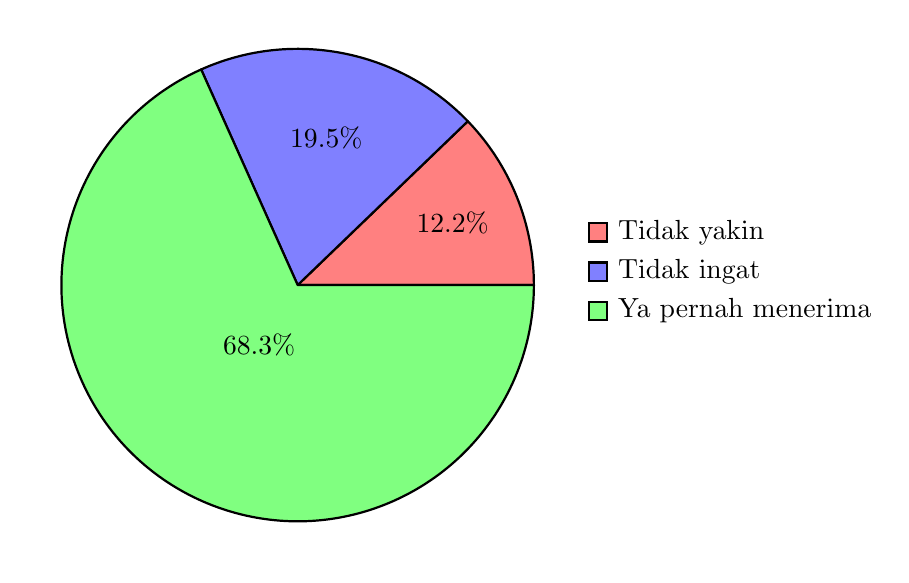
\begin{tikzpicture}
    \pie[
      text=legend,
      radius=3,
      color={red!50, blue!50, green!50}
    ]{
      12.2/Tidak yakin,
      19.5/Tidak ingat,
      68.3/Ya pernah menerima
    }
  \end{tikzpicture}
  \caption{Persentase Responden yang Pernah Menerima Email Phishing}
  \label{fig:phishing_experience}
\end{figure}

Dalam survei ini, kami meminta responden untuk mengidentifikasi "pesan email
yang mencurigakan atau berpotensi berbahaya yang Anda terima di masa lalu." 315
responden yang memenuhi syarat tidak dapat mengidentifikasi email, dan 311
responden yang memenuhi syarat dapat melakukannya. Kuota hanya diterapkan pada
responden yang memenuhi syarat yang mengingat email tersebut, dan responden
diberi insentif untuk mengingat email tersebut agar dapat berpartisipasi dalam
survei dan menerima pembayaran insentif. Tujuan kami bukan untuk menemukan
seberapa umum phishing di antara kelompok demografis yang berbeda, dan sampel
ini tidak boleh diartikan sebagai pengukuran prevalensi phishing. Namun, ini
menunjukkan bahwa sekitar 50\% dari orang-orang non-ahli dalam pool subjek
Qualtrics memiliki cerita tentang email phishing tertentu yang mereka terima,
yang menunjukkan betapa luasnya pengalaman dengan email-email ini.

Hampir semua pertanyaan yang tersisa dalam survei kemudian meminta responden
untuk memberikan lebih banyak detail tentang insiden spesifik di mana mereka
menerima email yang mereka pilih untuk diceritakan kepada kami: apa yang
terjadi saat mereka menerimanya, apa yang mereka perhatikan, dan bagaimana
mereka menanganinya? Dalam sebagian besar makalah ini, kami melaporkan
statistik tentang tanggapan terhadap pertanyaan pilihan ganda.

Berdasarkan temuan dari Wash \cite{tigaempat}, kami mengorganisir survei
berdasarkan enam aktivitas berbeda yang perlu dilakukan seseorang untuk
mengenali email phishing: 1) Memperhatikan aspek-aspek email; 2) Membentuk
ekspektasi tentang apa yang seharusnya dan tidak seharusnya ada dalam email; 3)
Menjadi curiga terhadap email; 4) Menyelidiki email; 5) Memutuskan apakah email
mencurigakan atau tidak; dan 6) Bertindak berdasarkan keputusan tersebut.

Enam aktivitas ini memberikan cara bagi kami untuk menggambarkan apa yang
umumnya terjadi ketika seseorang menerima email phishing, dan untuk melihat
pola dalam apa yang mereka perhatikan dan apa yang mereka lakukan. Kami
mengorganisir deskripsi temuan kami dalam makalah ini di sekitar enam aktivitas
berbeda ini.

\subsubsection{Insiden}

Setiap peserta diminta untuk menjawab pertanyaan tentang satu insiden yang
mereka alami. Kami mulai dengan menggambarkan jenis insiden yang dilaporkan
oleh responden. Setiap insiden adalah email yang diterima peserta dan dianggap
mencurigakan atau berpotensi berbahaya. Semua insiden ini mewakili email yang
berhasil melewati pertahanan teknis dan masuk ke kotak masuk peserta, sehingga
tidak termasuk email phishing yang berhasil difilter oleh perlindungan phishing
teknis. Namun, email-email ini tidak seragam; responden melaporkan menerima
berbagai jenis email phishing yang berbeda.

Kami meminta setiap responden untuk mengidentifikasi daftar kemungkinan
insiden/email yang memenuhi syarat, dan kemudian meminta mereka untuk memilih
satu yang "mudah diingat detailnya" dan kemudian menjawab lebih banyak
pertanyaan tentang yang satu itu. Kami memiliki total lima pertanyaan yang
mencoba memahami secara luas tentang apa email-email ini — satu pertanyaan di
awal yang meminta responden untuk merangkum insiden, satu pertanyaan di akhir
yang meminta responden untuk menjelaskan seluruh insiden, dan kemudian tiga
pertanyaan yang meminta deskripsi singkat, 5-kata tentang insiden yang dipilih.
Di sini kami menggunakan deskripsi 5-kata ini untuk menggambarkan jenis insiden
yang dilaporkan orang.

Ketika diminta untuk merangkum insiden di awal survei, responden merespons
dengan rata-rata 21 kata (median: 17 kata). Dalam ringkasan ini, responden
sebagian besar melaporkan fakta tentang email yang mereka terima, dengan
kata-kata yang paling umum adalah email (39\% responden), akun (17\%), uang
(15\%), tautan (13\%) dan menerima (11\%).

Selain ringkasan, kami meminta responden, "Dalam sekitar lima kata" untuk
menggambarkan apa yang membuat email mencurigakan, apa yang membuat email sulit
untuk dipahami, dan apa yang diminta email tersebut untuk mereka lakukan.
Responden melaporkan bahwa mereka curiga terutama melihat alamat email/pengirim
atau karena melibatkan uang. Email-email tersebut sebagian besar meminta
responden untuk mengklik tautan (22\%), untuk uang (17\%), atau untuk
"informasi" (14\%). Bersama-sama, ringkasan ini menunjukkan bahwa sebagian
besar cerita phishing adalah tentang masalah ekonomi (uang) atau meminta atau
memberikan informasi.

Sekitar 81\% responden menunjukkan bahwa mereka merasa mudah mengingat email
semacam itu. Email-email yang dipilih responden untuk dijawab tersebar luas
dalam waktu: 24\% responden menerimanya dalam minggu terakhir; 30\% dalam bulan
terakhir (tetapi bukan minggu terakhir); 25\% dalam tahun terakhir (tetapi
bukan bulan terakhir); dan 15\% lebih dari setahun yang lalu. Dalam pengkodean
manual, kami mengkodekan cerita insiden lengkap untuk informasi tentang siapa
pengirim email yang diklaim. Ini bukan siapa yang sebenarnya mengirim email,
tetapi siapa yang berpura-pura menjadi pengirim email. 44\% menunjukkan bahwa
email tersebut berasal dari kelompok atau organisasi, dan 25\% menunjukkan
bahwa email tersebut tampaknya berasal dari individu. Dalam 30\% cerita,
peserta menunjukkan bahwa mereka memiliki hubungan sebelumnya dengan pengirim
yang diklaim, dan 14\% cerita peserta secara eksplisit menyatakan bahwa mereka
tidak memiliki hubungan sebelumnya. 76\% dari hubungan sebelumnya adalah dengan
kelompok atau organisasi; menunjukkan bahwa email yang berpura-pura berasal
dari organisasi lebih mungkin dilihat sebagai bagian dari hubungan sebelumnya.

Sebagai contoh cerita tentang email dari organisasi yang peserta memiliki
hubungan sebelumnya, pertimbangkan cerita berikut tentang email dari
Amazon.com:

\textbf{Cerita P233}: \textit{menerima email yang tampaknya berasal dari amazon. Email tersebut memiliki nama dan alamat saya tetapi mengatakan saya berutang uang untuk pembelian. Saya tidak membeli apa pun untuk sementara waktu sehingga itu tampak aneh. Email tersebut memiliki kesalahan ejaan dan tautan yang aneh. Saya melihat email tersebut dengan cermat, kemudian memeriksa akun amazon saya di situs web mereka. Tidak ada apa pun di sana tentang pesanan atau utang uang.}

Pengirim sebenarnya bervariasi secara luas di seluruh cerita: sekitar 12\%
mengatakan itu adalah bank atau lembaga keuangan, 8\% mengatakan email tersebut
tampaknya berasal dari orang asing, 4\% dari pemerintah, dan 2\% dari
organisasi dukungan IT.

Dalam pengkodean manual cerita, kami juga mengkodekan untuk jenis informasi apa
yang diminta. 30\% cerita menyebutkan bahwa penerima email akan menerima
semacam barang berharga (uang, hadiah, tawaran pekerjaan, dll.), dan 19\%
cerita melaporkan bahwa email meminta penerima untuk mengirim uang. 19\% cerita
menyebutkan bahwa email meminta informasi pribadi, 10\% cerita meminta
informasi teknis seperti nama pengguna atau kata sandi, dan 10\% cerita meminta
informasi keuangan seperti nomor rekening bank, nomor kartu kredit, dll. Ini
menunjukkan bahwa responden kami menerima email dengan berbagai permintaan,
tanpa jenis permintaan tertentu yang sangat umum. Apa yang dianggap pengguna
akhir sebagai phishing sangat beragam, dan pelatihan yang berfokus terutama
pada petunjuk mungkin melewatkan kelas pesan email yang menonjol bagi pengguna
akhir sebagai berpotensi berbahaya.

\subsection{Memperhatikan}

\subsubsection{Apa yang diperhatikan orang dalam email}

Saat seseorang membaca email, mereka tidak dapat memperhatikan dan mengingat
semua tentang email tersebut. Sebaliknya, hal-hal dalam email yang paling mudah
mereka pahami dan hubungkan adalah yang paling mudah diperhatikan dan diingat
\cite{satudelapan}. Kami bertanya kepada responden "Aspek apa dari email yang
menonjol bagi Anda?" dan memungkinkan mereka untuk mencentang semua yang
berlaku. Jawaban atas pertanyaan ini menunjukkan kepada kami, untuk email-email
phishing yang dicurigai ini, aspek apa dari email yang paling penting bagi
responden, karena mereka adalah yang paling mudah diingat.

Jauh lebih banyak, aspek yang diperhatikan oleh jumlah orang terbesar adalah
bahwa email tersebut mencakup permintaan untuk tindakan. 76\% responden
memperhatikan ini tentang email tersebut. Ini sesuai dengan penelitian
sebelumnya yang menunjukkan bahwa orang cenderung menggunakan email sebagai
daftar tugas \cite{tigaenam}; mereka dengan cepat fokus pada apa yang diminta
email untuk mereka lakukan. Ini juga sesuai dengan temuan Wash \cite{tigaempat}
bahwa permintaan untuk tindakan (tautan tindakan) adalah pemicu penting bagi
para ahli.

Aspek kedua yang paling umum diperhatikan dari email adalah tentang apa email
tersebut, dengan 52\% responden memperhatikan ini. Topik email, dan apakah
topik tersebut relevan dengan penerima email, umumnya dianggap sebagai aspek
penting dari phishing. Data ini mendukung gagasan tersebut, dan menunjukkan
bahwa ini adalah sesuatu yang dengan cepat dapat diidentifikasi dan diingat
oleh orang-orang tentang email.

Banyak pekerjaan sebelumnya tentang phishing telah berfokus pada "pembeda
konklusif": aspek-aspek email yang dapat membantu penerima untuk secara
konklusif membedakan email yang sah dari email phishing, atau setidaknya sangat
menunjukkan phishing. Misalnya, pelatihan phishing biasanya berfokus pada aspek
seperti URL yang tidak sesuai dalam tautan, urgensi dalam permintaan tindakan,
atau tata bahasa/ejaan yang buruk. Namun, Wash menekankan bahwa ketika para
ahli mengidentifikasi email phishing di kotak masuk mereka sendiri, mereka
malah mencari ketidaksesuaian yang lebih kecil, yaitu hal-hal yang tampak aneh
tentang email tersebut, tetapi tidak selalu menunjukkan phishing dan tentu saja
tidak cukup untuk secara konklusif mengidentifikasi phishing.

Dua hal pertama yang diperhatikan responden — permintaan untuk tindakan dan
topik email — tidak secara konklusif menunjukkan bahwa email tersebut adalah
pesan phishing, dan biasanya bukan bagian dari pelatihan phishing. Sebaliknya,
mereka hanya menunjukkan bahwa ada sesuatu yang aneh tentang email tersebut.
Namun, bagi beberapa orang, itu mungkin sudah cukup. Misalnya, pertimbangkan
cerita ini:

\textbf{Cerita P19}: \textit{Saya mendapat email Jumat lalu dari salah satu perusahaan yang kami bekerja untuk mereka yang membayar kami untuk menyediakan layanan bagi mereka dan saya segera bisa tahu itu adalah email palsu karena perusahaan yang menyamar sebagai pengirim email adalah perusahaan yang membayar kami, kami tidak membayar mereka. Saya menelepon perusahaan yang kami bekerja untuk dan melaporkannya kepada mereka sehingga mereka tahu seseorang mencoba menyamar sebagai mereka.}

Dua aspek email berikutnya yang paling umum diperhatikan lebih sering dikaitkan
dengan identifikasi phishing: tautan dalam email (44\%), kesalahan atau
kualitas buruk (41\%). Ini sering ditemukan dalam email phishing (terutama
jenis email phishing yang mungkin dapat dideteksi oleh non-ahli dalam sampel
kami).

Sekitar 38\% responden melaporkan bahwa nama pengirim menonjol bagi mereka.
Aspek email lainnya, seperti lampiran, gambar, format, atau panjang email,
diperhatikan oleh kurang dari 20\% responden, meskipun semuanya penting bagi
sebagian kecil pengguna. Temuan ini menunjukkan bahwa orang tampaknya secara
alami memperhatikan tindakan dan topik email jauh lebih banyak daripada mereka
memperhatikan pembeda konklusif seperti URL atau kesalahan ketik. Ini penting,
karena seseorang tidak dapat menggunakan fitur untuk mendeteksi phishing
kecuali mereka pertama kali memperhatikan fitur tersebut.

\section{Discussion}

\subsubsection{Humans Identify Phishing Differently}
Sistem email modern melibatkan beberapa lapisan perlindungan terhadap serangan
phishing. Banyak pengirim email menyertakan pemeriksaan phishing saat email
dikirim. Sebagian besar sistem email menyertakan setidaknya satu, dan sering
kali lebih dari satu sistem teknis yang menyaring email yang diyakini sebagai
spam atau phishing. Banyak dari sistem ini juga memberi label email sebagai
kemungkinan phishing, sebagai peringatan kepada pengguna (misalnya, sistem
email Google \cite{dualima}). Dan pengguna akhir membaca email dan membuat
penentuan legitimasi mereka sendiri.

Model Swiss Cheese dari Reason tentang penyaringan \cite{duadelapan}
menunjukkan bahwa ketika ada rantai filter seperti ini, filter bekerja paling
baik ketika setiap filter bekerja pada prinsip yang berbeda atau menggunakan
informasi yang berbeda dari filter lain dalam rantai. Jika dua filter
menggunakan informasi yang sama (misalnya, alamat email pengirim) dengan cara
yang sama, maka lubang di keju akan sejajar dan email berbahaya yang lolos dari
satu filter juga kemungkinan besar akan lolos dari yang lain. Namun, jika dua
filter menggunakan informasi yang berbeda, atau beroperasi pada informasi
dengan cara yang sangat berbeda, maka setiap filter kemungkinan akan menangkap
pesan yang terlewatkan oleh filter lainnya, dan menyertakan kedua filter
membuat sistem lebih tangguh terhadap serangan daripada hanya menyertakan satu.

Dalam makalah ini, kami menyajikan bukti bahwa filter terakhir ini – manusia
yang membaca email dan menentukan apakah email tersebut sah – beroperasi dengan
cara yang sangat berbeda, menggunakan pengetahuan dan kemampuan yang berbeda,
daripada hampir semua filter teknis. Kami menemukan bahwa manusia memiliki
informasi penting yang tidak dimiliki oleh filter phishing teknis. Mereka
mengandalkan keakraban mereka dengan email terkait yang diterima di masa lalu
(72\%) dan harapan mereka terhadap email yang masuk (95\%) untuk memahami dan
menjadi curiga terhadap email phishing. Pengetahuan ini sangat kontekstual dan
sangat unik bagi setiap individu dan pengalaman mereka. Selain itu, manusia
menggunakan pengetahuan mereka tentang apa yang biasa ada dalam email yang
mereka terima di masa lalu untuk melihat bagian informasi yang tidak terduga
dan hilang dalam email baru. Informasi ini sangat penting untuk mendeteksi
serangan phishing zero-day, yang jarang terdeteksi oleh solusi teknis
\cite{satudua}.

Responden kami mampu memperhatikan sifat email (misalnya 78\% memperhatikan
bahwa itu bersifat pribadi) dan akun email tempat email diterima. Ini
memerlukan pengetahuan tentang semua akun email yang dimiliki seseorang dan
jenis komunikasi yang diharapkan di setiap akun berdasarkan bagaimana dan apa
yang dipilih orang tersebut untuk menggunakan setiap akun. Sangat kompleks dan
menantang bagi filter teknis untuk memperoleh pengetahuan semacam itu dan
menerapkannya dengan tepat, kecuali mereka mengawasi individu.

Kedua, kami menemukan bahwa manusia memiliki kemampuan unik yang mereka gunakan
untuk mengidentifikasi pesan phishing, yang tidak dimiliki oleh filter teknis.
94\% responden non-ahli mampu mengidentifikasi tindakan apa yang diminta email
untuk mereka lakukan, dan lebih dari tiga perempat mengatakan mereka secara
eksplisit memperhatikan hal ini tentang email tersebut. Permintaan untuk
tindakan tidak umum menjadi bagian dari banyak filter spam dan phishing, dan
ketika ada, sering kali terbatas dalam cakupan terutama oleh masalah bahasa
(misalnya memeriksa apakah email berisi tautan ke halaman login dan
memverifikasi apakah halaman login tersebut sah \cite{duatiga}). Bahkan
non-ahli sangat peka terhadap permintaan ini dan dapat mengidentifikasinya
dengan percaya diri.

Saat menyaring, manusia juga memiliki kemampuan investigasi yang tidak dimiliki
oleh filter teknis: mereka dapat memilih untuk mengambil waktu tambahan dan
mencari lebih banyak informasi dari sumber pihak ketiga. Sejumlah responden
kami menunjukkan bahwa mereka akan meminta nasihat dari rekan kerja atau
mencoba menghubungi pengirim email yang diklaim.

Di atas adalah kemampuan dan pengetahuan yang dimiliki manusia, tetapi tidak
dimiliki oleh filter phishing teknis. Mengikuti logika Model Swiss Cheese,
mengandalkan kombinasi penyaringan manusia dan teknis lebih baik daripada hanya
mengandalkan salah satu. Dalam beberapa tahun terakhir, organisasi telah lebih
mengandalkan deteksi phishing otomatis. Temuan kami menunjukkan bahwa
mengurangi keragaman filter dapat membuat sistem rentan terhadap phishing, dan
bahwa mendekati pelatihan pengguna akhir dengan cara yang berbeda dapat
memperkuat strategi untuk mencegah kerugian dari phishing.

Banyak saran tentang phishing dalam komunitas TI melibatkan pencegahan pesan
agar tidak pernah sampai ke pengguna akhir \cite{satuempat}, daripada mencoba
mendidik pengguna akhir. Karena pengguna akhir mampu menyaring pesan dengan
cara yang sangat berbeda dari filter teknis, akan lebih berharga untuk
menghabiskan sebagian uang dan sumber daya untuk meningkatkan kemampuan
pengguna akhir untuk memiliki peran signifikan dalam mendeteksi pesan phishing.
Terlalu banyak pelatihan phishing yang berfokus pada detail teknis (seperti
parsing URL [19, 30]) atau perubahan perilaku (seperti tidak mengklik [20,
    35]), daripada mencoba memperkuat kemampuan yang unik bagi manusia. Dalam
makalah ini, kami telah menyajikan bukti beberapa pengetahuan dan kemampuan
yang dimiliki manusia yang dapat dimanfaatkan untuk meningkatkan pelatihan dan
deteksi phishing, misalnya membentuk harapan untuk email dan meminta informasi
dari orang lain.

Seperti yang ditunjukkan oleh Model Swiss Cheese, dalam serangkaian filter,
menempatkan semua sumber daya Anda ke dalam satu lapisan filter dengan
mengesampingkan yang lain menghilangkan manfaat yang Anda dapatkan dari
strategi pertahanan berlapis. Seringkali lebih baik memiliki dua filter yang
tidak sempurna yang beroperasi pada prinsip atau informasi yang berbeda
daripada memiliki satu filter yang sangat dioptimalkan tetapi terbatas.

\subsubsection{Similar to Expert Phishing Detection?}

Temuan kami juga memiliki implikasi untuk mengidentifikasi kesamaan antara
deteksi email phishing oleh pengguna ahli dan non-ahli. Wash \cite{tigaempat}
melakukan studi mendetail tentang bagaimana orang mendeteksi email phishing.
Studi tersebut dilakukan dengan para ahli IT – orang-orang dengan pelatihan IT
dan pengalaman profesional yang memungkinkan mereka untuk berhasil mendeteksi
email phishing. Kami memperluas model tersebut, dan mendasarkan banyak
pertanyaan kami pada model yang diperluas tersebut, sebagian untuk mencoba
menentukan apakah fitur-fitur dari model tersebut juga ada dalam cara non-ahli
mendeteksi phishing.

Dalam makalah ini, kami dapat memvalidasi bagian dari modelnya dengan populasi
non-ahli. Wash juga menunjukkan bahwa selain keahlian IT, menjadi pekerja
pengetahuan dapat memberikan keahlian dalam mengelola email yang relevan dengan
deteksi phishing. Sampel kami bukan ahli IT, dan juga bukan pekerja pengetahuan
yang secara konstan berurusan dengan email.

Secara khusus, kami dapat memvalidasi bahwa non-ahli memang memiliki ekspektasi
tentang apa yang seharusnya ada dalam email dan memperhatikan ketika hal-hal
tersebut berbeda. Kami juga dapat memvalidasi bahwa bahkan pada non-ahli,
perhatian orang terfokus pada apa yang diminta email untuk mereka lakukan;
hampir semua orang dalam studi kami dapat mengidentifikasi permintaan apa yang
dibuat oleh email tersebut. Kami memvalidasi bahwa non-ahli kami melaporkan
bahwa mereka sering memiliki firasat bahwa ada sesuatu yang salah dengan email
tersebut, membantu mereka menjadi curiga. Kami dapat memvalidasi bahwa orang
sering mengambil langkah eksplisit untuk menyelidiki email yang mereka anggap
mencurigakan. Dan kami dapat memvalidasi bahwa non-ahli mampu secara konklusif
memutuskan apakah email tersebut adalah email phishing atau tidak. Ini
mendukung implikasi bahwa keahlian tentang kotak masuk email seseorang adalah
aspek penting dan belum dimanfaatkan dalam pelatihan deteksi phishing.

Kami tidak dapat memvalidasi semua aspek model Wash dengan non-ahli. Secara
khusus, model Wash mencakup urutan kronologis dari tahap-tahap – pertama
pemahaman, kemudian kecurigaan, kemudian bertindak. Studi kami adalah survei
dan tidak dapat menentukan urutan kronologis dari kejadian, dan dengan
demikian, kami tidak yakin bahwa hal-hal tersebut terjadi pada non-ahli dalam
urutan yang diusulkan oleh Wash.

\subsubsection{Implications for Phishing Prevention}
Pengguna email melakukan investigasi yang kompleks terhadap email yang
mencurigakan sebelum mereka menentukan apakah email tersebut adalah phishing,
tetapi pelatihan dan teknologi saat ini tidak mendukung investigasi ini. Temuan
kami menunjukkan bahwa pelatihan phishing dapat lebih mendukung investigasi
pengguna dengan mendorong pengguna untuk menunda tindakan hingga menyelesaikan
investigasi mereka dan mendorong pengguna email untuk memanfaatkan kemampuan
rekan (seperti meminta bantuan teman). Selain itu, perusahaan yang mengirim
email dapat menyediakan dukungan gaya helpdesk untuk membantu pengguna
menentukan apakah perusahaan benar-benar mengirim email tersebut kepada
pengguna. Klien email dapat lebih mendukung investigasi dengan menyertakan
tombol "bantu saya memecahkan masalah email ini", dengan saran kontekstual
untuk investigasi.

\section{Limitations}
Makalah ini tentang orang-orang, kognisi mereka, dan bagaimana mereka berhasil
mendeteksi phishing. Ini bukan tentang email phishing. Survei bukanlah metode
yang baik untuk mengumpulkan data kebenaran dasar tentang email phishing yang
sebenarnya atau kegagalan deteksi, karena bias seleksi dan ingatan yang tidak
sempurna.

Mengingat email phishing mendorong pengingatan kejadian tertentu, memungkinkan
survei untuk menyelidiki proses yang digunakan orang untuk mendeteksi email
phishing di kotak masuk mereka. Jawaban yang kami terima hanya tentang satu
insiden spesifik ini, dan tidak selalu mewakili insiden lain yang dialami orang
tersebut; namun, di antara responden, jawaban ini mewakili berbagai jenis
insiden phishing yang dihadapi oleh non-ahli. Penelitian sebelumnya hampir
secara eksklusif berfokus pada kegagalan deteksi dan memperbaiki kegagalan
tersebut; kami sebaliknya melihat apa yang bekerja dengan baik dalam deteksi
phishing dan apa yang harus didukung.

Karena ini adalah survei, kami hanya dapat mengajukan pertanyaan rinci tentang
hal-hal yang kami ketahui sebelumnya. Kami mendasarkan pertanyaan survei kami
pada investigasi Wash tentang deteksi phishing oleh ahli \cite{tigaempat}. Kami
tidak dapat menentukan apakah non-ahli juga menggunakan metode tambahan yang
tidak ada pada ahli Wash. Artinya, kami berusaha untuk mengetahui metode ahli
mana yang juga digunakan oleh non-ahli, tetapi kami tidak dapat mempelajari
metode non-ahli yang unik untuk non-ahli. Oleh karena itu, kami tidak mengklaim
bahwa metode ini adalah deskripsi komprehensif tentang bagaimana non-ahli
mengidentifikasi phishing; sebaliknya, kami mengkarakterisasi beberapa metode
yang mereka gunakan.

\section{Conclusion}
Phishing adalah ancaman keamanan siber yang dialami banyak orang; hampir
setengah dari orang yang memenuhi syarat untuk survei kami dapat
mengidentifikasi setidaknya satu email phishing spesifik yang mereka terima.
Orang-orang ini memiliki cerita tentang pengalaman phishing yang dapat mereka
bagikan dengan orang lain, dan kami menduga cerita-cerita ini membentuk bagian
penting dari bagaimana pengguna email belajar tentang phishing.

Kami menemukan bahwa banyak teknik yang digunakan para ahli untuk
mengidentifikasi phishing \cite{tigaempat}, seperti memperhatikan
ketidaksesuaian kecil, membentuk ekspektasi tentang bagaimana email seharusnya
terlihat dan memperhatikan perbedaan dari ekspektasi tersebut, serta menjadi
curiga dan menyelidiki email lebih dekat, juga hadir dalam cara non-ahli
mendeteksi email phishing.

Kami juga menemukan bahwa banyak informasi yang digunakan non-ahli saat
mengidentifikasi phishing tidak dapat direplikasi oleh sistem deteksi phishing
teknis. Pengguna akhir mengetahui tujuan (bisnis, pribadi) dari akun email
tempat mereka menerima email, dan memperhatikan fakta tersebut. Mereka tahu
apakah email tersebut diharapkan, dan dapat membandingkannya dengan email lain
yang serupa yang pernah mereka terima di masa lalu (email phishing sering kali
terasa familiar). Selain itu, non-ahli ini memiliki kemampuan investigasi,
seperti menunda merespons email dan meminta konfirmasi atau informasi lebih
lanjut dari pengirim, yang tidak dimiliki oleh filter phishing teknis.
Menargetkan pelatihan phishing di masa depan untuk meningkatkan penggunaan
pengetahuan unik ini dan memperluas penggunaan kemampuan ini kemungkinan akan
menghasilkan peningkatan dalam perlindungan phishing.

\section*{Acknowledgments}
This should be a simple paragraph before the References to thank those individuals and institutions who have supported your work on this article.

\begin{thebibliography}{1}
  \bibliographystyle{IEEEtran}

  \bibitem{satu}
  Jeremy Bryans and Budi Arief. Security implications of structure. In Structure for Dependability: Computer-Based Systems from an Interdisciplinary Perspective, pages 217–227. Springer, 2006.

  \bibitem{dua}
  Deanna D Caputo, Shari Lawrence Pfleeger, Jesse D
  Freeman, and M Eric Johnson. Going spear phishing:
  Exploring embedded training and awareness. IEEE
  Security & Privacy, 12(1):28–38, 2013.

  \bibitem{tiga}
  Debra L. Cook, Vijay K. Gurbani, and Michael Daniluk.
  Phishwish: a simple and stateless phishing filter. Secu-
  rity and Communication Networks, 2(1):29–43, 2009.

  \bibitem{empat}
  Lorrie Faith Cranor. Can phishing be foiled? Scientific
  American, 299(6):104–111, 2008.

  \bibitem{lima}
  Nicola Davinson and Elizabeth Sillence. It won’t happen
  to me: Promoting secure behaviour among internet users.
  Computers in Human Behavior, 26(6):1739–1747, 2010.

  \bibitem{enam}
  Julie S. Downs, Mandy Holbrook, and Lorrie Faith Cra-
  nor. Behavioral response to phishing risk. In Proceed-
  ings of the Anti-Phishing Working Groups 2nd Annual
  ECrime Researchers Summit, eCrime ’07, pages 37–44,
  New York, NY, USA, 2007. Association for Computing
  Machinery.

  \bibitem{tujuh}
  Julie S Downs, Mandy B Holbrook, and Lorrie Faith
  Cranor. Decision strategies and susceptibility to phish-
  ing. In Proceedings of the second symposium on Usable
  privacy and security, pages 79–90, 2006.

  \bibitem{delapan}
  Serge Egelman, Lorrie Faith Cranor, and Jason Hong.
  You’ve been warned: An empirical study of the effective-
  ness of web browser phishing warnings. In Proceedings
  of the SIGCHI Conference on Human Factors in Com-
  puting Systems, CHI ’08, pages 1065–1074, New York,
  NY, USA, 2008. Association for Computing Machinery.

  \bibitem{sembilan}
  Ian Fette, Norman Sadeh, and Anthony Tomasic. Learn-
  ing to detect phishing emails. In Proceedings of the 16th
  International Conference on World Wide Web, WWW
  ’07, pages 649–656, New York, NY, USA, 2007. Asso-
  ciation for Computing Machinery.

  \bibitem{satunol}
  Joshua T Goodman, Paul S Rehfuss, Robert L Rounthwaite, Manav Mishra, Geoffrey J Hulten, Kenneth G Richards, Aaron H Averbuch, Anthony P Penta, and Roderict C Deyo. Phishing detection, prevention, and notification, October 16 2012. US Patent 8,291,065.

  \bibitem{satusatu}
  The Radicati Group, ``Email statistics report 2019-2023 executive summary,'' Technical report, The Radicati Group, 2019.

  \bibitem{satudua}
  Ryan Heartfield and George Loukas. A taxonomy of
  attacks and a survey of defence mechanisms for seman-
  tic social engineering attacks. ACM Computing Surveys
  (CSUR), 48(3):1–39, 2015.

  \bibitem{satutiga}
  Thorsten Holz, Christian Gorecki, Konrad Rieck, and
  Felix C Freiling. Measuring and detecting fast-flux ser-
  vice networks. In The Network and Distributed System
  Security Symposium (NDSS), 2008.

  \bibitem{satuempat}
  Jason Hong. The state of phishing attacks. Communications of the ACM, 55(1):74, Jan 2012.

  \bibitem{satulima}
  Scott D Johnson, Jeffrey W Flesher, and Shih-Ping
  Chung. Understanding troubleshooting styles to im-
  prove training methods. In American Vocational Associ-
  ation Convention. ERIC, Dec 1995.

  \bibitem{satuenam}
  Y. Joshi, S. Saklikar, D. Das, and S. Saha. Phishguard:
  A browser plug-in for protection from phishing. In
  2008 2nd International Conference on Internet Multimedia Services Architecture and Applications, pages 1–6,
  2008.

  \bibitem{satutujuh}
  Mahmoud Khonji, Youssef Iraqi, and Andrew Jones.
  Phishing detection: a literature survey. IEEE Communications Surveys & Tutorials, 15(4):2091–2121, 2013.

  \bibitem{satudelapan}
  Gary Klein. Sources of Power: How People Make Decisions. MIT Press, 1998.

  \bibitem{satusembilan}
  Ponnurangam Kumaraguru, Steve Sheng, Alessandro
  Acquisti, Lorrie Faith Cranor, and Jason Hong. Teach-
  ing johnny not to fall for phish. ACM Transactions on
  Internet Technology (TOIT), 10(2):1–31, 2010.

  \bibitem{duanol}
  Robert LaRose, Nora J. Rifon, and Richard Enbody. Pro-
  moting personal responsibility for internet safety. Com-
  munications of the ACM, 51(3):71–76, March 2008.

  \bibitem{duasatu}
  Eric Lipton, David E Sanger, and Scott Shane. The Perfect Weapon: How Russian Cyberpower Invaded the U.S. The New York Times, dec 2016.

  \bibitem{duadua}
  MacEwan University. University Discovers Online Fraud. Press Release, 2017. https://www.macewan.ca/wcm/MacEwanNews/PHISHING\_ATTACK.

  \bibitem{duatiga}
  L. A. T. Nguyen, B. L. To, H. K. Nguyen, and M. H.
  Nguyen. A novel approach for phishing detection using
  url-based heuristic. In 2014 International Conference
  on Computing, Management and Telecommunications
  (ComManTel), pages 298–303, 2014.

  \bibitem{duaempat}
  US Bureau of Labor Statistics. Employment–
  population ratio, Retrieved Feb, 2021. https:
  //www.bls.gov/charts/employment-situation/
  employment-population-ratio.htm.

  \bibitem{dualima}
  Rob Pegoraro. We keep falling for phishing emails,
  and google just revealed why. Fast Company,
  2019. https://www.fastcompany.com/90387855/
  we-keep-falling-for-phishing-emails-and-
  google-just-revealed-why.

  \bibitem{duaenam}
  Justin Petelka, Yixin Zou, and Florian Schaub. Put your
  warning where your link is: Improving and evaluating
  email phishing warnings. In Proceedings of the 2019
  CHI Conference on Human Factors in Computing Sys-
  tems, CHI ’19, pages 1–15, New York, NY, USA, 2019.
  Association for Computing Machinery.

  \bibitem{duatujuh}
  Emilee Rader, Rick Wash, and Brandon Brooks. Stories
  as informal lessons about security. In Proceedings of
  the Eighth Symposium on Usable Privacy and Security
  (SOUPS), pages 1–17, 2012.

  \bibitem{duadelapan}
  James Reason. Human Error. Cambridge University
  Press, 1990.

  \bibitem{duasembilan}
  Ozgur Koray Sahingoz, Ebubekir Buber, Onder Demir,
  and Banu Diri. Machine learning based phishing de-
  tection from urls. Expert Systems with Applications,
  117:345 – 357, 2019.

  \bibitem{tiganol}
  Steve Sheng, Bryant Magnien, Ponnurangam Ku-
  maraguru, Alessandro Acquisti, Lorrie Faith Cranor, Ja-
  son Hong, and Elizabeth Nunge. Anti-phishing phil: the
  design and evaluation of a game that teaches people not
  to fall for phish. In Proceedings of the 3rd Symposium
  on Usable Privacy and Security (SOUPS), pages 88–99,
  2007.

  \bibitem{tigasatu}
  Rebecca Smith. How a U.S. Utility Got Hacked. Wall Street Journal, Dec 2016.

  \bibitem{tigadua}
  Symantec. Internet Security Threat Report. Technical Report February, 2019.

  \bibitem{tigatiga}
  Verizon. 2019 Data Breach Investigations Report. Technical report, 2019.

  \bibitem{tigaempat}
  Rick Wash. How experts detect phishing scam emails. Proceedings of the ACM: Human Computer Interaction, CSCW(160), October 2020.

  \bibitem{tigalima}
  Rick Wash and Molly M Cooper. Who provides phish-
  ing training? facts, stories, and people like me. In Pro-
  ceedings of the 2018 CHI Conference on Human Factors
  in Computing Systems, pages 1–12, 2018.

  \bibitem{tigaenam}
  Steve Whittaker, Victoria Bellotti, and Jacek Gwizdka.
  Email in personal information management. Communi-
  cations of the ACM, 49(1):68–73, January 2006.

  \bibitem{tigatujuh}
  Weining Yang, Aiping Xiong, Jing Chen, Robert W.
  Proctor, and Ninghui Li. Use of phishing training to
  improve security warning compliance: Evidence from a
  field experiment. In Proceedings of the Hot Topics in Sci-
  ence of Security: Symposium and Bootcamp, HoTSoS,
  pages 52–61, New York, NY, USA, 2017. Association
  for Computing Machinery.

\end{thebibliography}

\newpage

\section{Biography Section}
If you have an EPS/PDF photo (graphicx package needed), extra braces are needed
around the contents of the optional argument to biography to prevent the LaTeX
parser from getting confused when it sees the complicated
$\backslash${\tt{includegraphics}} command within an optional argument. (You
can create your own custom macro containing the
$\backslash${\tt{includegraphics}} command to make things simpler here.)

\vspace{11pt}

\bf{If you include a photo:}\vspace{-33pt}
\begin{IEEEbiography}[{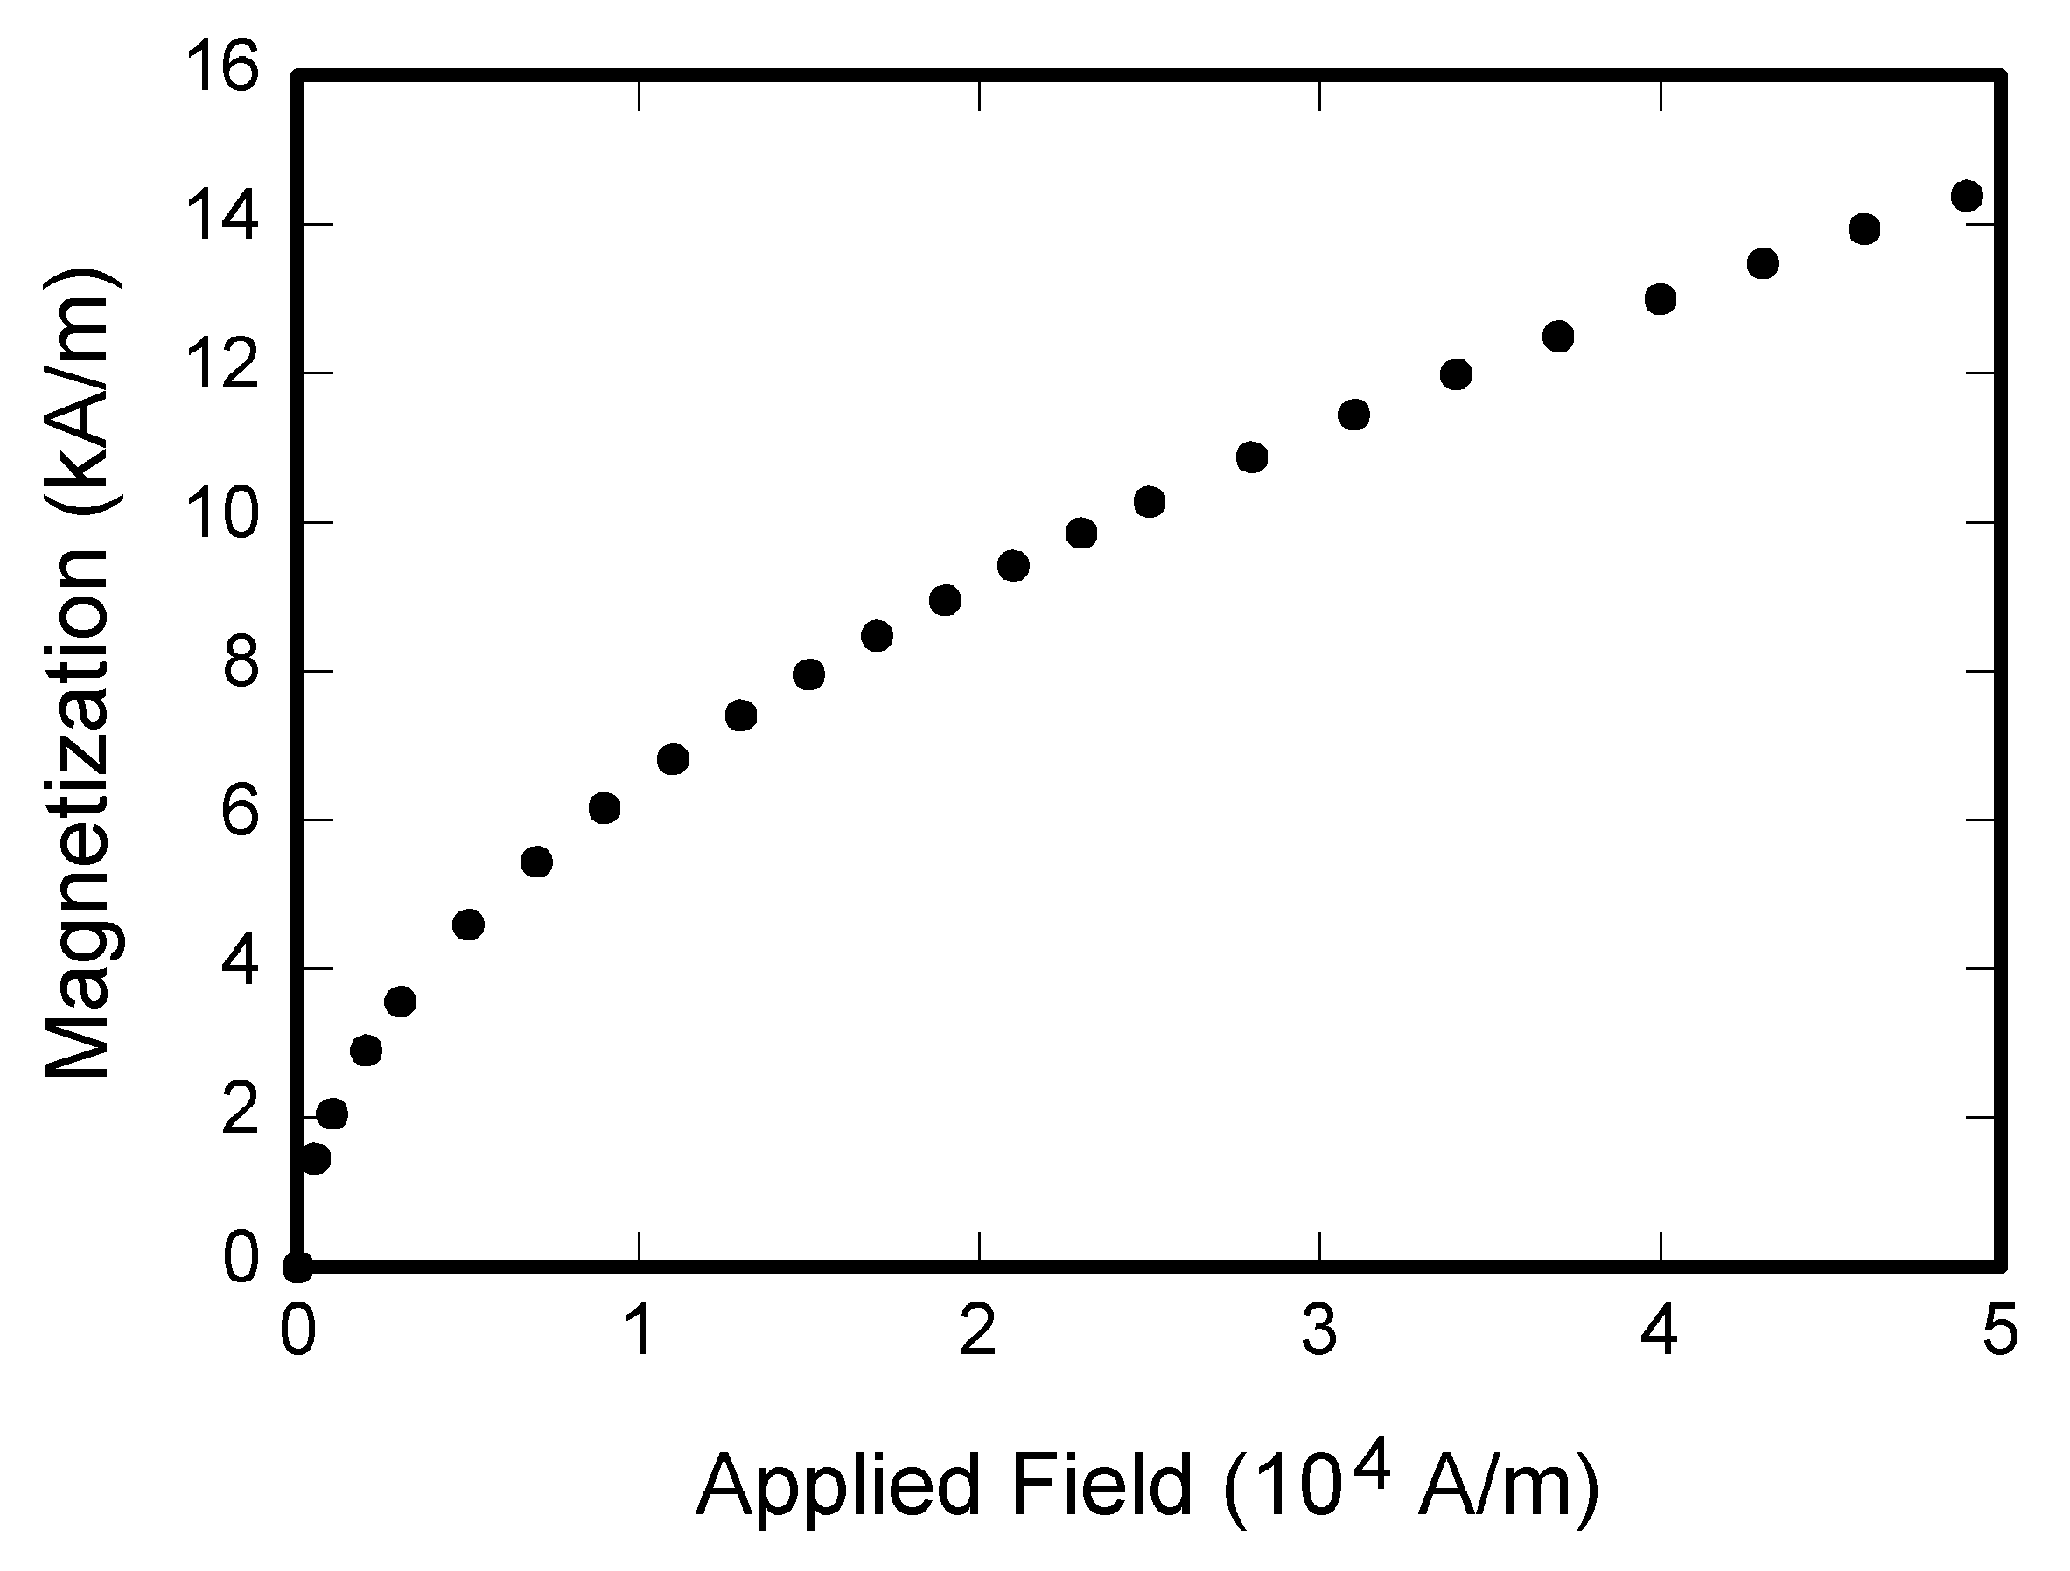
\includegraphics[width=1in,height=1.25in,clip,keepaspectratio]{fig1}}]{Michael Shell}
  Use $\backslash${\tt{begin\{IEEEbiography\}}} and then for the 1st argument use $\backslash${\tt{includegraphics}} to declare and link the author photo.
  Use the author name as the 3rd argument followed by the biography text.
\end{IEEEbiography}

\vspace{11pt}

\bf{If you will not include a photo:}\vspace{-33pt}
\begin{IEEEbiographynophoto}{John Doe}
  Use $\backslash${\tt{begin\{IEEEbiographynophoto\}}} and the author name as the argument followed by the biography text.
\end{IEEEbiographynophoto}

\vfill

\end{document}

